\documentclass{jsarticle}

%----------------------------------
% 文章の中に 画像を入れるための設定
%----------------------------------
\usepackage[dvipdfmx]{graphicx}

%----------------------------------
% 自分の作る文章の題
%----------------------------------
\title{上腕三頭筋の働きと鍛え方}

%---------------------------------- 
% 文書を作った日
%----------------------------------
\date{\today}

%----------------------------------
% 自分の名前を入れる
%----------------------------------
\author{山 根 千 佳}

%---------------------------------------------------
% 文書のスタイルを決める設定
%---------------------------------------------------
\usepackage[height=26cm,width=16cm]{geometry}

%-----------------------------------
% 以上で下準備は終わりです.
% ここから表示される文章を作成していきます.
%-----------------------------------
\begin{document}

%----------------------------------------
% 文章に上に、上記で記述したタイトル、
% 文書を作成した日にち, 著者の名前を書き込みます.
%
% (注)\maketitle をはずせば, タイトル, 日にち,著者名は文書に挿入されません.
%----------------------------------------

\maketitle

%--------------------------------------------
% 主な内容はここから
%--------------------------------------------

\section{目的}
上腕二頭筋及び上腕三頭筋は、どちらも肩から肘の間に存在する筋肉であるが、それらの知名度には差がある。
上腕二頭筋は、重い物を持ち上げると、力こぶとして見ることができ、そのトレーニング方法をイメージしやすい。
しかし、上腕三頭筋は、場所がイメージしにくく、その働きやトレーニング方法をイメージしにくい。
そこで、本レポートは、上腕三頭筋の性質を計測実験により調べ、得られたデータからその働きやトレーニング方法について考察する。

\section{実験方法}
被験者は、膝をついた状態で座り、腕を床と水平に繰り返し曲げ伸ばしした。
計測は、腕の伸縮をゆっくり行った場合と、早く行った場合との2パターンについて行った。

\subsection{人の腕の軌道の計測}
実験には、MotionCaptureを用いた。
具体的には、被験者の運動の様子を真上からカメラで撮影し、肩、肘、手首の3点を追跡することで、各関節の位置座標の変化を計測した。

\subsection{筋電データの計測}
上腕二頭筋および上腕三頭筋に筋電計を貼り付け、各筋電データを取得した。

\subsection{取得データの解析}
筋電データには、1〜40Hzのバンドパスフィルタをかけた。このデータをもとに、時刻$t$における筋肉の活動度$a(t)$を、
$$a(t) = \frac{1}{ΔT} \int_{t-\frac{ΔT}{2}}^{t+\frac{ΔT}{2}} |E(t)|dt $$
として求めた。つまり、ある時刻$t$における筋肉の活動度を、その周辺ΔT個のデータ値を平均することで求めた。
これにより、ノイズの影響を少なくすることを考えた。もう少し具体的に言うと、ある時刻$t$において急激な上昇が見られた場合に、それをノイズとするか、
統計的に有意な上昇と捉えるかを、区間ΔTの範囲を変更することで、各自決定できるようにした。

また、取得した軌道データには、計測条件などの文字列が含まれていたため、データ部(数値)だけを取り出してファイル出力した。
そして、そのデータを、グラフ作成に用いた。

\clearpage
\section{結果}

\begin{figure}[h]
	\begin{center} %センタリングする
		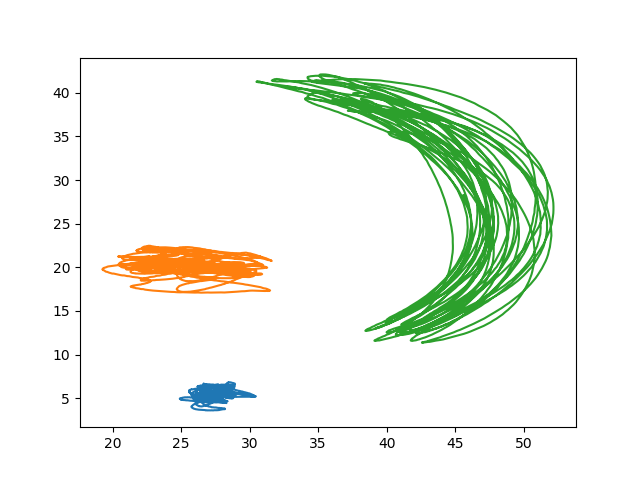
\includegraphics[width=10cm]{graph_image/slow.png}
		\caption{腕の3関節の軌道} %タイトルをつける
		\label{kidou} %ラベルをつけ図の参照を可能にする
	\end{center}
\end{figure}
図\ref{kidou}はゆっくりと腕の曲げ伸ばし運動を行った場合の、各関節の位置変化を示す。
水色が肩、オレンジが肘、黄緑が手首の位置変化を示している。
この図から、今回の実験では、手首におけるY軸方向の動きが激しいことがわかる。

\begin{figure}[!h]
	\begin{center}
		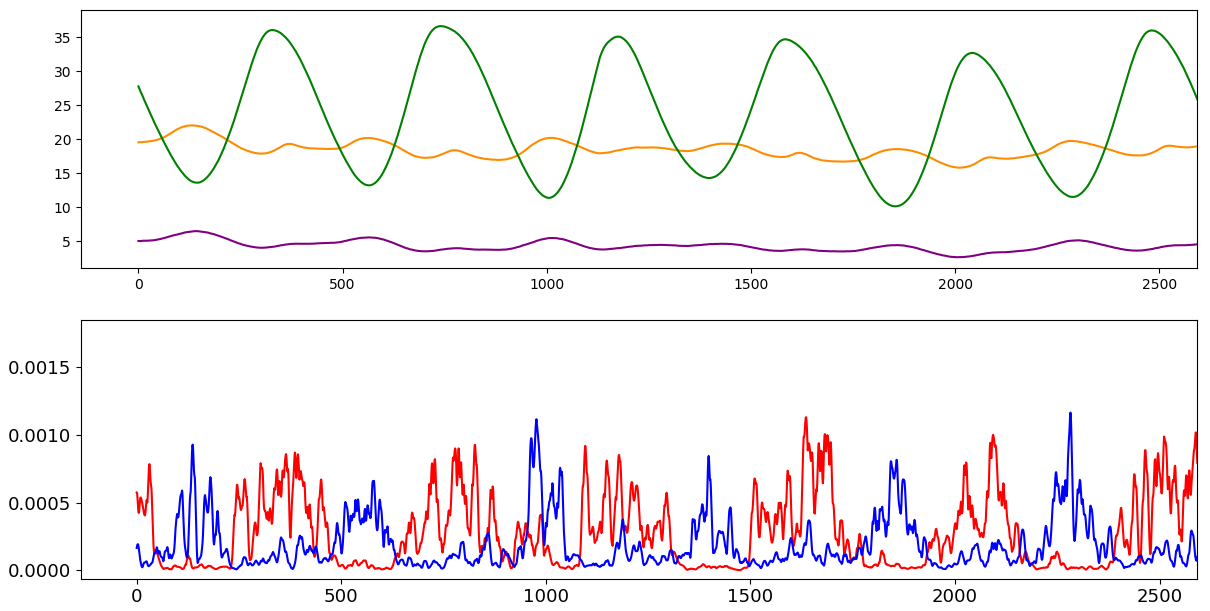
\includegraphics[width=17cm]{graph_image/fast_final.png}
		\caption{腕の曲げ伸ばし速度が速い時の筋電データ}
		\label{fast}
	\end{center}
\end{figure}
\clearpage

\begin{figure}[!h]
	\begin{center}
		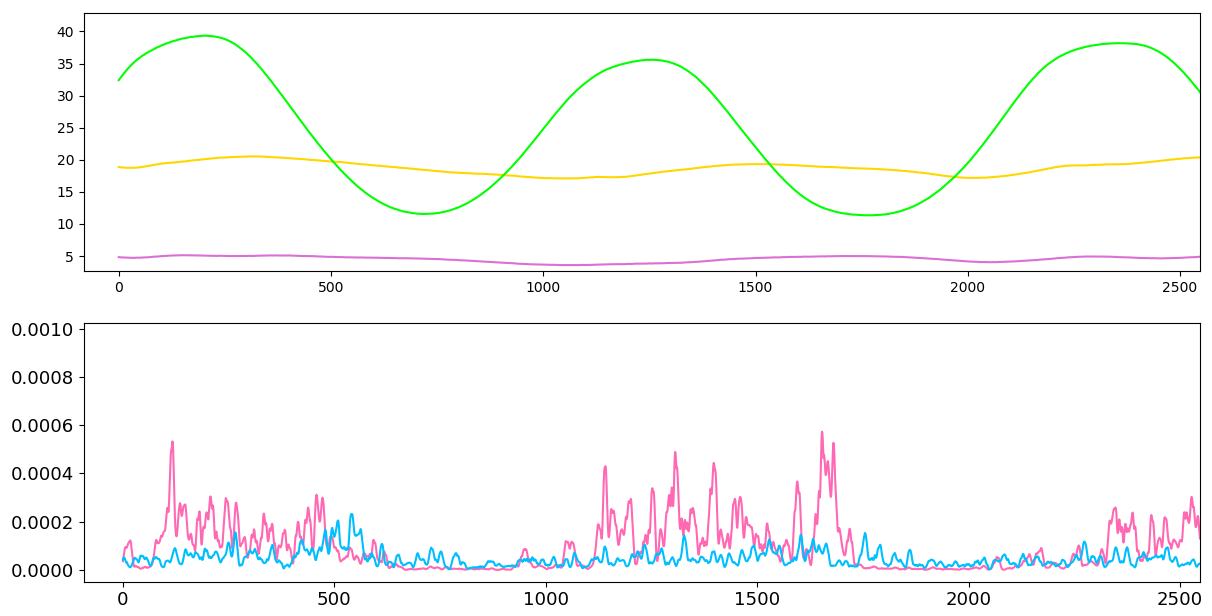
\includegraphics[width=17cm]{graph_image/slow_final.png}
		\caption{腕の曲げ伸ばし速度が遅い時の各関節のY軸方向への位置変化。}
		\label{slow}
	\end{center}
\end{figure}

図\ref{fast}では、上段が腕の曲げ伸ばし運動を速く行った場合のY軸方向の位置変化である。紫が肩、オレンジが肘、緑が手首の位置変化を示す。
下段は、赤が上腕二頭筋、青が上腕三頭筋の筋電データであり、縦軸は活動電位(単位はmV)、横軸は時間(単位はms)である。
図\ref{slow}では、上段が腕の曲げ伸ばし運動を遅く行った場合のY軸方向の位置変化である。薄紫が肩、黄色が肘、黄緑が手首の位置変化を示す。
下段は、ピンクが上腕二頭筋、水色が上腕三頭筋の筋電データであり、縦軸は活動電位(単位はmV)、横軸は時間(単位はms)である。
図\ref{fast}および図\ref{slow}上段のグラフを比較する。当然であるが、腕を速く動かした方が、遅く動かしたときよりも位置変化の周波数が高くなっている。
 
図\ref{fast}において、上腕二頭筋の筋電図は、Y軸方向の手首の動きと逆位相の形となった。つまり、腕が曲がる(手首がY軸下向きに移動する)ほど、より多くの筋繊維で活動電位が発生していることがわかる。また、速い腕の曲げ伸ばしでは、上腕二頭筋と上腕三頭筋のグラフがほぼ完全な逆位相になっていた。

一方、図\ref{slow}を見ると、遅い腕の曲げ伸ばしでは、上腕二頭筋と上腕三頭筋のグラフに位相のずれが生じているようにみえるが逆位相ではなかった。また、上腕二頭筋と上腕三頭筋のグラフの形が、図\ref{fast}ほどに似ておらず、上腕二頭筋の振幅が大きくなった後でも、それほど上腕三頭筋の振幅に変化が見られない部分も見られた。

また、両者のグラフを比較すると、上腕二頭筋の方が上腕三頭筋よりも大きな活動電位を発生させる傾向が見られた。また、腕を速く曲げ伸ばしした場合、遅く曲げ伸ばしした場合に比べて、高い活動電位が見られた。


\section{考察}

本を読んでいると、上腕二頭筋は、腕を曲げる働きがあり、上腕三頭筋は腕を伸ばす働きがあるという情報があった\cite{reference}。しかし、腕の伸縮が遅い場合、上腕三頭筋には、上腕二頭筋に対応した大きな振幅を持つ部分が見られないこともあり、比較的平坦に近いグラフが出力された。このグラフでは、振幅は0に近かったが、完全に0となることはほとんどなかった。
私はこのことから、腕の伸縮が遅い場合のグラフでは、腕を伸ばすための活動電位に加えて、肩から腕までの部分を地面と水平に保持する筋力を発生させるための活動電位を見ているのではないかと考えた。つまり、上腕三頭筋には、肘を伸ばす役割の他に、肩から肘までの位置を固定・維持する役割があるのではないかと考えた。

また、腕を速く動かした場合の上腕三頭筋の筋電データが、Y軸方向における手首の位置変化から、腕を伸ばすときに上腕三頭筋での活動電位が大きくなることが確認できた。
これらのことから、上腕三頭筋を鍛えるためには、腕の曲げ伸ばし運動に加えて、肩から腕の位置固定を物理的に難しくするトレーニング(例えば、肩から腕までの部位に思いリングのようなものをかけた状態で腕を素早く曲げ伸ばしするなど)が有効なのではないかと考えられる。

\section{参考文献}
\begin{thebibliography}{9}
	\bibitem{reference} 「3D 踊る肉単」 河合良訓,原島広至 pp.xiv
\end{thebibliography}
%--------------------------------------------
% 文章これまで.
%--------------------------------------------
\end{document}
